% ═══════════════════════════════════════════════════════════════════════════════
\section{Structural Constraints on GVC Integration}
\label{sec:constraints}
% ═══════════════════════════════════════════════════════════════════════════════

\subsection{A Framework for Constraint Analysis}

The distinction between \textit{binding constraints} and \textit{peripheral constraints} is analytically important for policy prioritisation. Hausman, Rodrik, and Velasco's (2008) growth diagnostics framework argues that economies face a ``tree'' of potential constraints on growth, and that policy resources are most productively allocated to the \textit{binding} constraint --- the one whose relaxation yields the greatest increment to growth --- rather than distributed across all observed constraints simultaneously. Applied to Uzbekistan's GVC integration challenge, the question is: which constraint, if relaxed, would most immediately accelerate the transition from captive to relational GVC participation?

This section assesses five candidate binding constraints: landlockedness and transit costs; energy and utility infrastructure; financial sector depth; currency regime residual uncertainty; and political economy constraints on reform deepening. For each, the magnitude of the constraint is quantified where data permit, and a counterfactual comparison with comparator economies is drawn.

\subsection{Constraint 1: Landlockedness and Transit Costs}

\citet{limao2001} originally estimated that landlocked countries face trade costs approximately 55\% higher than coastal comparators, all else equal. More recent literature corroborates this structural penalty, demonstrating that geographical disadvantages profoundly constrain a nation's ability to participate in high-value, time-sensitive GVCs. For Uzbekistan --- doubly landlocked, surrounded only by other landlocked states (Kazakhstan, Kyrgyzstan, Tajikistan, Afghanistan, Turkmenistan) --- this penalty is compounded: the minimum number of border crossings to reach deep-water ports is three (via Kazakhstan to Russia to the Black Sea, or via Turkmenistan to Iran to the Persian Gulf), versus zero for Vietnam and one for Thailand.

Empirical measurement of Uzbekistan's transit cost premium is presented in Table~\ref{tab:transit_costs}.

\begin{table}[H]
 \centering
 \caption{Transit Cost Comparison: Uzbekistan versus Benchmark Economies (2022)}
 \label{tab:transit_costs}
 \small
 \begin{tabular}{@{}lccccc@{}}
 \toprule
 Country & Container cost (USD/20ft) & Transit days & Border crossings & LPI score & Trade/GDP \\
 \midrule
 Uzbekistan & \$3,400 & 25--40 & 3--4 & 2.57 & 52\% \\
 Vietnam & \$890 & 3--5 & 0 & 3.27 & 210\% \\
 Thailand & \$750 & 2--4 & 0 & 3.41 & 125\% \\
 Kazakhstan & \$2,100 & 15--25 & 2--3 & 2.85 & 65\% \\
 Ethiopia$^*$ & \$2,800 & 20--35 & 1 & 2.31 & 28\% \\
 \bottomrule
 \end{tabular}
 \\\smallskip
 \small * Ethiopia included as a landlocked comparator (GVC-active in garments). Container cost = estimated door-to-port cost for standard 20ft container (export). Transit days = typical delay from factory gate to destination port. Source: World Bank Logistics Performance Index 2023; IFC Cost of Doing Business; author compilation.
\end{table}

The cost premium is stark: exporting a container from Uzbekistan costs approximately four times more than from Vietnam and carries 5--8 times the transit time. This makes Uzbekistan structurally non-competitive in any GVC task where: (i) just-in-time delivery is required (electronics, automotive), (ii) product perishability is relevant (agro-processing beyond dried products), or (iii) final buyer specifications require rapid replenishment cycles (fast fashion). The sectors in which Uzbekistan remains potentially competitive despite transit costs are those with high value-to-weight ratios (precision instruments, pharmaceuticals, ICT hardware) or with high labour cost sensitivity relative to logistics costs (low-complexity textiles, basic automotive components for the CIS market).

Three infrastructure investments could materially reduce this constraint. The China-Kyrgyzstan-Uzbekistan (CKU) railway, under negotiation since the 1990s and with construction beginning in 2024, would reduce rail transit time from Uzbekistan to Chinese ports by approximately 30\%. However, analysts of the Belt and Road Initiative warn that such infrastructure must be carefully managed to ensure it facilitates symmetrical trade rather than merely extractive outflows. The Trans-Caspian International Transport Route (Middle Corridor) --- connecting China via Kazakhstan, the Caspian Sea, Azerbaijan, Georgia, and Turkey to European markets --- has seen freight volumes grow 88\% in 2022--2023 following Russia-related rerouting and could accommodate Uzbek export cargo at scale if Uzbekistan develops feeder rail connections. Air freight from Navoiy (the Navoiy model discussed in Section~\ref{sec:sez}) offers a partial solution for high-value products.

\subsection{Constraint 2: Energy and Utility Infrastructure}

Manufacturing productivity depends critically on reliable and affordable energy supply. Uzbekistan has experienced periodic electricity shortages since 2020, driven by the deterioration of Soviet-era power generation infrastructure and growing domestic demand from a young, urbanising population. Table~\ref{tab:energy} documents the energy constraint relative to comparators.

\begin{table}[H]
 \centering
 \caption{Energy Infrastructure: Uzbekistan and Comparators}
 \label{tab:energy}
 \small
 \begin{tabular}{@{}lcccc@{}}
 \toprule
 Indicator & Uzbekistan & Vietnam & Thailand & China \\
 \midrule
 Electricity access (\%, 2022) & 100 & 100 & 100 & 100 \\
 Power outages (hrs/year, mfg. firms) & 120 & 18 & 4 & 6 \\
 Electricity tariff (USD/kWh, industry) & \$0.06 & \$0.09 & \$0.12 & \$0.08 \\
 Electr. losses in distribution (\%) & 18.3 & 9.8 & 6.2 & 5.4 \\
 Renewable share of generation (\%) & 12 & 48 & 18 & 28 \\
 \bottomrule
 \end{tabular}
 \\\smallskip
 \small Power outages: World Bank Enterprise Surveys (latest available year). Source: World Bank WDI; IEA; World Bank Enterprise Surveys.
\end{table}

Uzbekistan's electricity tariff for industry (\$0.06/kWh) is the lowest in the comparator set --- a genuine cost advantage for energy-intensive manufacturing. But 120 hours of power outages per year (versus 18 in Vietnam and 4 in Thailand) imposes hidden costs far in excess of the tariff advantage: manufacturers facing unreliable power must invest in backup generation, cannot run continuous-process manufacturing at full capacity, and face product quality risks in precision manufacturing operations. The 18.3\% distribution loss rate reflects ageing grid infrastructure and represents a structural inefficiency that limits the power available to industry even when generation capacity is technically sufficient.

The planned energy sector reform programme --- including privatisation of distribution companies, tariff rebalancing (currently below cost recovery), and investment in renewable generation (solar: 5~GW by 2030) --- would address these constraints, but at the cost of higher industrial electricity prices that would partially offset the current tariff advantage.

\subsection{Constraint 3: Financial Sector Depth and Trade Finance}

Export-oriented manufacturing requires access to trade finance (letters of credit, export credit guarantees) and medium-term investment finance for capital equipment acquisition. Uzbekistan's banking sector remains shallow by regional standards: domestic credit to the private sector stood at 38\% of GDP in 2022 (Vietnam: 131\%; Thailand: 164\%), and the sector remains dominated by state-owned banks (NBU, Ipotekabank, Asaka Bank) that are subject to directed credit allocation rather than commercial lending criteria.

The practical consequence for GVC integration is twofold. First, domestic firms aspiring to become suppliers in Northeast Asian production networks cannot access the capital needed to upgrade equipment and certify to international quality standards. Second, foreign investors in SEZs face difficulty repatriating profits through formal banking channels, creating FX liquidity risk that discourages long-term equity commitment. The Central Bank of Uzbekistan's post-2017 liberalisation has reduced but not eliminated these frictions: the som became formally convertible in 2017, but large USD transactions still face informal scrutiny, and the forward exchange market is insufficiently liquid for corporate risk management purposes.

\subsection{Constraint 4: Political Economy of Reform Continuity}

A constraint less tractable to quantification but analytically important is the political economy of reform continuity. The Mirziyoyev reform programme was launched through presidential decree rather than through legislative process, creating a reform architecture that depends on sustained executive commitment rather than entrenched institutional rules. This creates two risks.

First, reform reversal risk: policies established by decree can be reversed by decree, particularly if they generate distributional losers (import-competing domestic industries, state enterprise managers, regional elites benefiting from rent allocation under the old system). Several episodes of partial policy reversal are already observable: export restrictions on copper and aluminium were reimposed in 2021--2022 under industrial policy rationales, partially contradicting the open trade commitments of the 2017 reforms.

Second, elite capture of SEZs: the rapid proliferation of FEZs and small industrial zones creates opportunities for politically connected firms to capture SEZ benefits (land, tax holidays, import duty exemptions) without generating the export-oriented manufacturing activity that justifies the fiscal cost. OECD (2022) documents several cases in Central Asian FEZs where the primary beneficiaries were domestic importers using zone status to avoid tariffs rather than exporters generating value addition.

These political economy constraints are not unique to Uzbekistan --- Vietnam and Thailand both experienced similar tensions between reform coalitions and rent-seeking incumbents. The difference is that Vietnam's WTO accession (2007) and Thailand's ASEAN obligations provided binding external commitment mechanisms that constrained reversal and reduced the space for elite capture. Furthermore, institutional economists observe that weak formal institutions can severely hinder long-term innovation and upgrading, forcing firms to rely on fragile informal networks. Uzbekistan's WTO accession process (observer status since 1994, active negotiations ongoing) represents the equivalent mechanism, and its acceleration should be treated as a first-order policy priority for this reason.

\subsection{Constraint Hierarchy and the Binding Constraint}

Figure~\ref{fig:constraint_heatmap} synthesises the constraint analysis into a prioritisation matrix, scoring each constraint on two dimensions: (i) severity (how large is the constraint's current effect on GVC integration potential?) and (ii) tractability (how amenable is the constraint to policy intervention within a 5--7 year horizon?).

\begin{figure}[H]
 \centering
 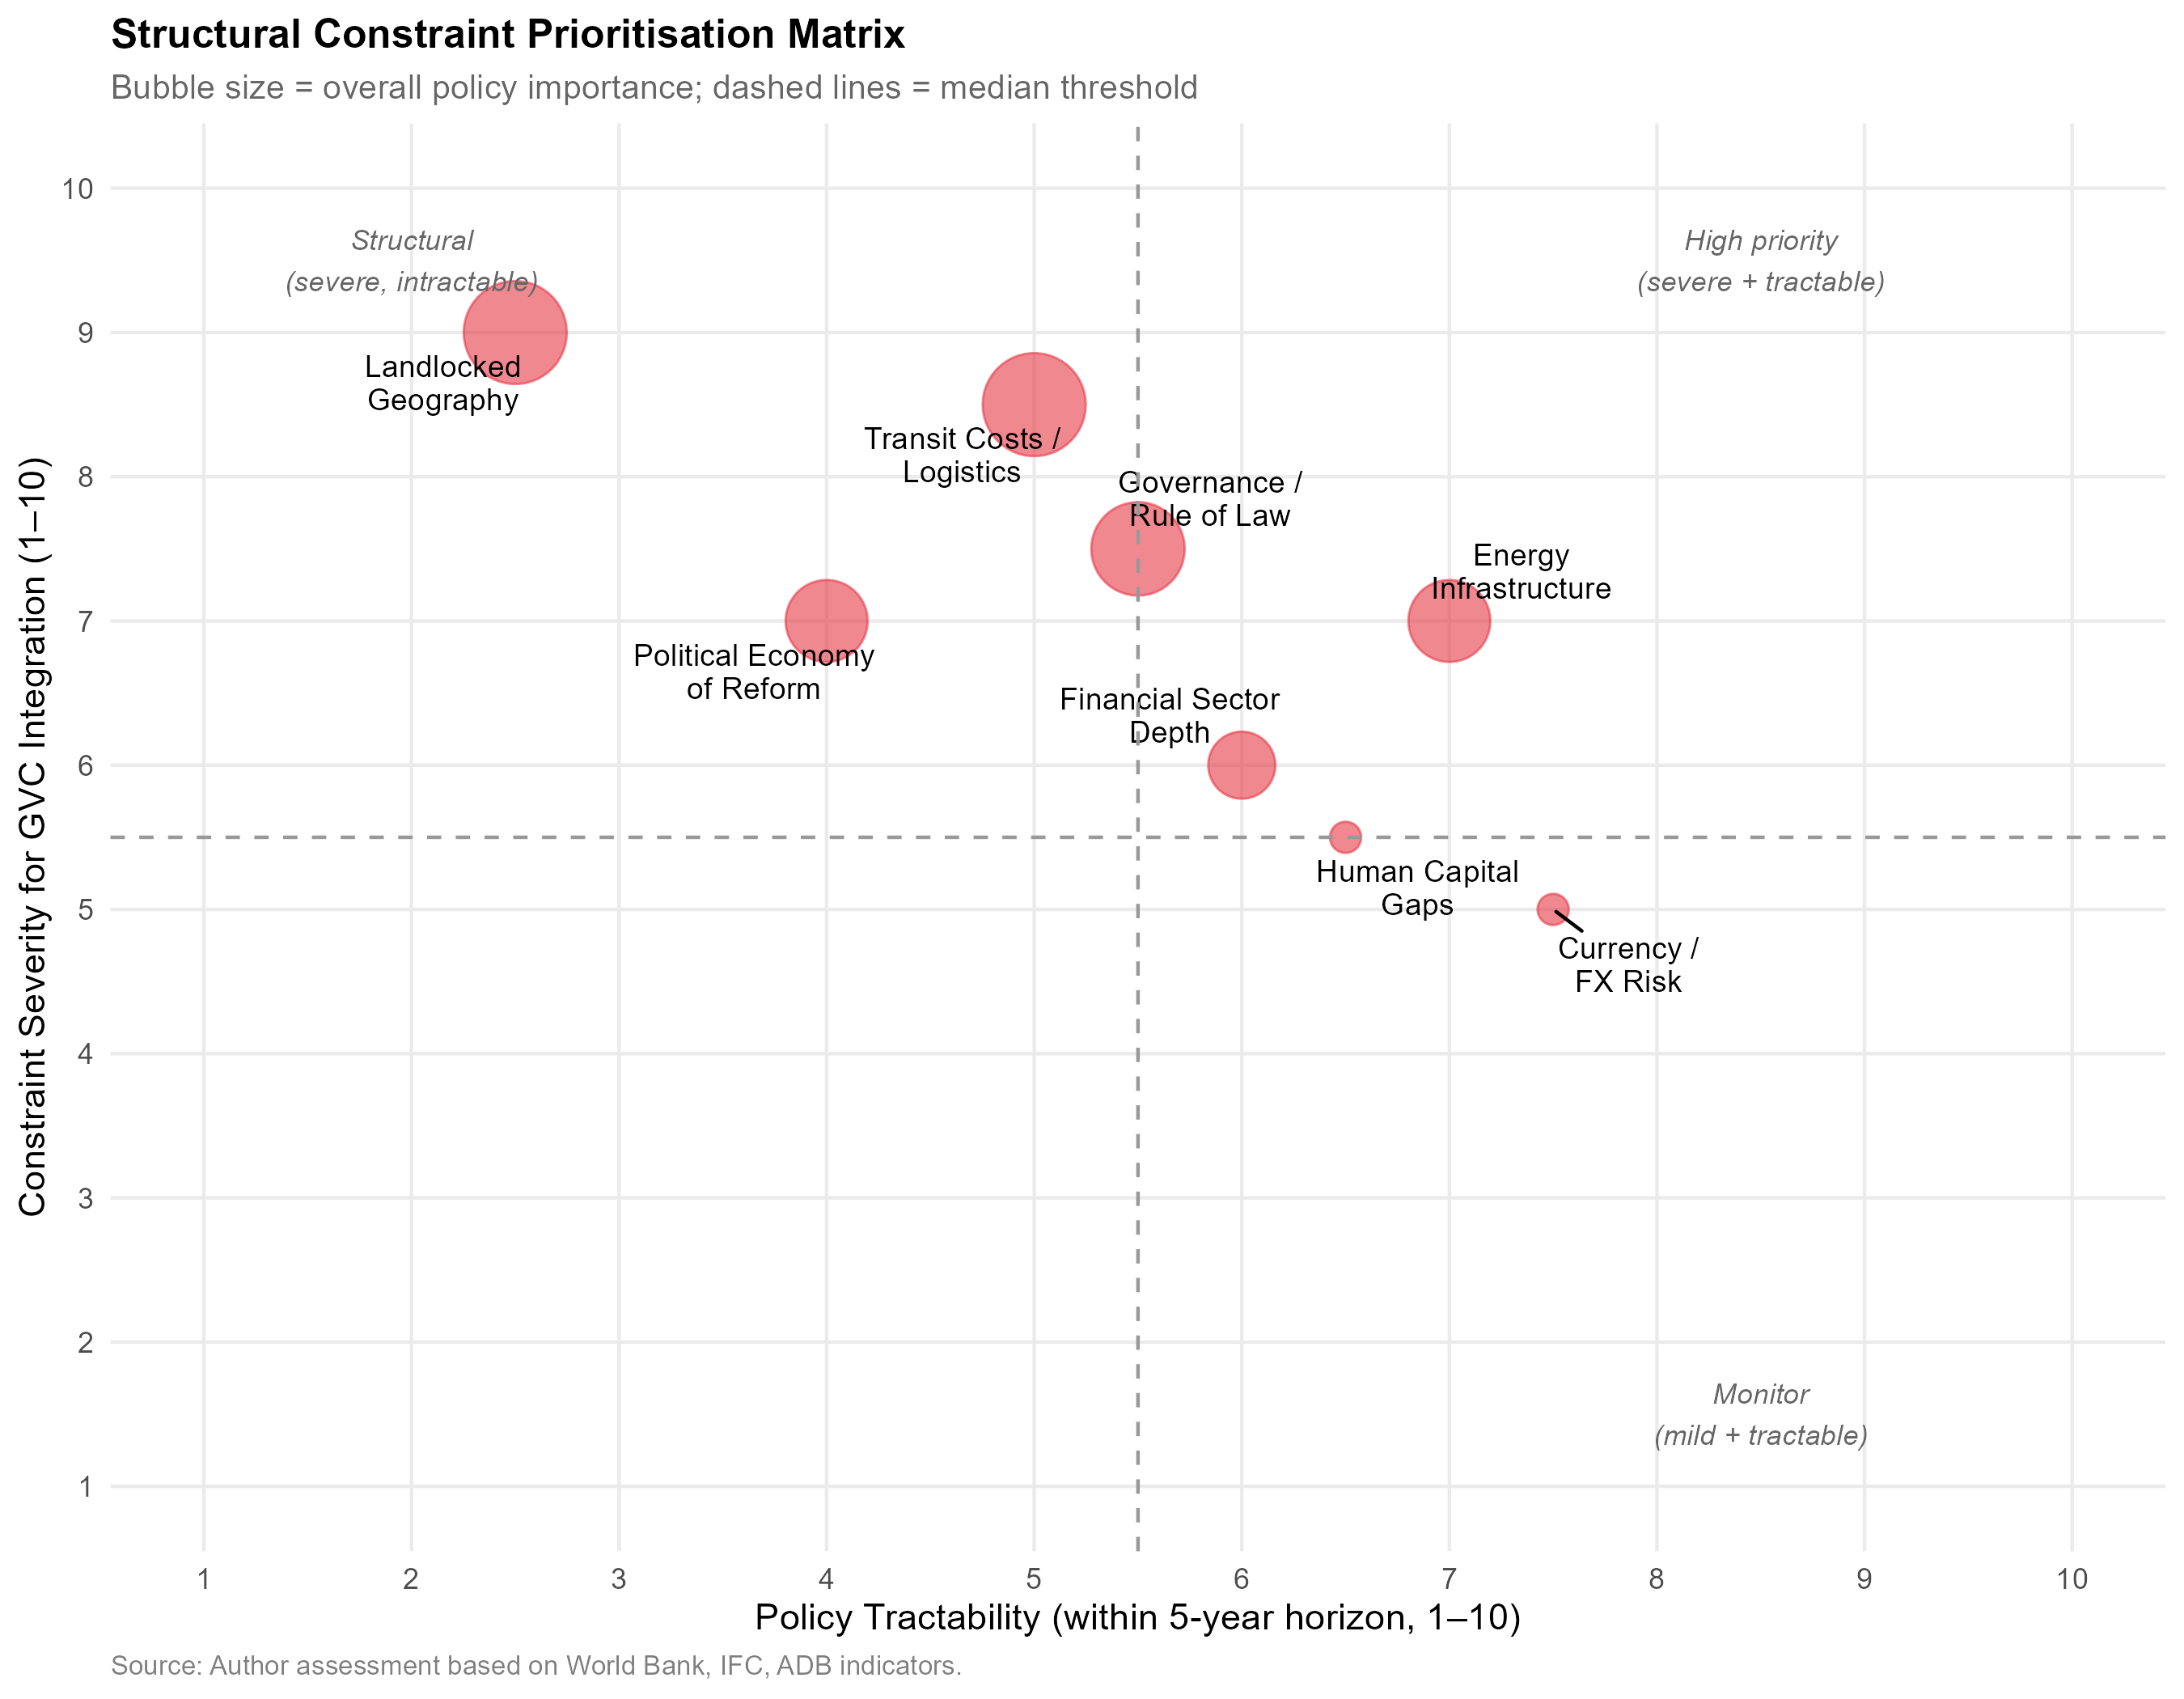
\includegraphics[width=0.88\textwidth]{figures/fig21_constraint_heatmap.png}
 \caption{Structural Constraint Prioritisation Matrix: Severity vs.\ Policy Tractability. Upper-left quadrant = severe and intractable; upper-right quadrant = severe but tractable (highest priority). Each constraint rated 0--10 on each dimension. Source: Author assessment based on World Bank, IFC, ADB data.}
 \label{fig:constraint_heatmap}
\end{figure}

The analysis places transit cost/logistics as the most severe constraint (score 8.5/10) but only partially tractable in the short run (score 5/10), given the dependence on multilateral infrastructure projects (CKU railway, Middle Corridor) outside Uzbekistan's unilateral control. Energy infrastructure is severe (7/10) but more tractable through domestic investment and tariff reform (tractability 7/10). Financial sector depth is moderately severe (6/10) and tractable through ongoing banking sector reform (6/10). Political economy constraints are severe (7/10) but have the lowest tractability (4/10), given their dependence on political will and external anchor mechanisms.

The growth diagnostics conclusion is that \textit{logistics and border-crossing efficiency} constitutes the nearest-term binding constraint amenable to policy action, followed by energy reliability. Both should take precedence in infrastructure investment sequencing over the proliferation of additional SEZs, which are unlikely to attract qualitatively superior FDI until the logistical infrastructure connecting them to export markets is improved.
